\documentclass[11pt]{article}
\usepackage{url,amsmath,setspace,amssymb,amsthm,fullpage}
\usepackage{algorithm,algorithmic,caption}
\usepackage{tikz}
\usetikzlibrary{arrows}
\usepackage[colorlinks=true]{hyperref}
\usepackage{bibentry}

% Scribe template modified from original created by UC Berkeley's EECS department

\newcommand{\heading}[5]{
   \renewcommand{\thepage}{#1-\arabic{page}}
   \noindent
   \begin{center}
   \framebox[\textwidth]{
     \begin{minipage}{0.9\textwidth} \onehalfspacing
       {\bf STAT 234 -- Sequential Decision Theory} \hfill #2

       {\centering \Large #5

       }\medskip

       {\it #3 \hfill #4}
     \end{minipage}
   }
   \end{center}
}

\newcommand{\scribe}[4]{\heading{#1}{#2}{Instructor:
Susan Murphy}{Scribe: #4}{Lecture #1: #3}}

\newtheorem{lemma}{Lemma}
\newtheorem{theorem}[lemma]{Theorem}
\newtheorem{proposition}[lemma]{Proposition}

\newtheorem{definition}{Definition}

\usepackage{bbm}

\newcommand\reals{\mathbb{R}} % real numbers
\newcommand\E[1]{\mathbb{E}\left[ #1 \right]} %expectation
\newcommand\prob[1]{\mathbb{P}\left( #1 \right)} %expectation
\DeclareMathOperator*{\argmax}{argmax} % argmax
\DeclareMathOperator*{\argmin}{argmin} % argmin
\newcommand\actions{\mathcal{A}} % set of actions
\newcommand\la{\mathcal{L}} % learning algorithm
\newcommand\history{\mathcal{H}} % history
\newcommand\regret{\mathcal{R}} % regret
\newcommand\distfam{\mathcal{D}} % distribution family
\newcommand\ind{\mathbbm{1}}  % indicator function
\newcommand\CDF{\mathrm{CDF}} % CDF
\newcommand\contexts{\mathcal{X}} % Contexts
\newcommand{\states}{\mathcal{S}} %states

\bibliographystyle{alpha}

\begin{document}

\scribe{9}{Feb.~20, 2018}{$Q$-Learning and SARSA}{Richard Ouyang}

\section{Reviewing Last Lecture (\texorpdfstring{$\boldsymbol{Q}$}{Q}-Learning)}

We began today's lecture by finishing up our discussion of $Q$-learning and its update rules. Recall that many statistical incremental algorithms are incremental versions of estimating equations. Another way to think about these algorithms is that there is a fixed point, and we are trying to iterate to the fixed point. Unfortunately, oftentimes there is not actually a fixed point.

\subsection{Bellman's Equation}

Recall that
\begin{align*}
Q^\pi(s, a) &= \E{R + \gamma \sum_{a} \pi(a | s')Q^\pi(s', a) | S = s, A = a} \\
&= (\mathcal{T}^\pi Q)^\pi(s,a).
\end{align*}
Interestingly, the expectation in the first line is not taken with respect to $\pi$. This occurs because we are considering the distribution of the reward given the state and action, neither of which depends on the policy $\pi$. Also note that $Q^\pi$ is a fixed point of $\mathcal{T}^\pi(Q) = Q$, so $Q^\pi$ satisfies this equality.

\subsection{Bellman's Optimality Equation}

Bellman's optimality equation underlies the batch operation of the TD(0) algorithm:

\begin{align*}
Q^{\pi^\star}(s,a) &= \E{R + \gamma + \max_{a'} Q^{\pi^\star}(s', a') | S = s, A = a}\\
&= (\mathcal{T}^\star Q)^{\pi^\star}(s,a).
\end{align*}

Analogous to the previous section, $Q^{\pi^\star}$ is the unique fixed point of $Q = \mathcal{T}^\star Q$. Note that $\mathcal{T}^\star$ is a slightly different operator than $\mathcal{T}^\pi$. 

\subsection{Batch Estimation}

In the batch version, $Q^{\pi^\star}$ solves
$$0 = \mathbb{P}_n\left[\sum_{t = 0}^{T - 1}\left(R_{t + 1} + \gamma \max_{a'} \hat{Q}^{\pi^\star}(S_{t + 1}, a') - \hat{Q}^{\pi^\star}(s, a)\right)\mathbbm{1}_{S_t=s,A_t=a}\right],$$
where $T$ is a geometric stopping time.

If we think of $Q$ as a matrix in which each row is a state and each column is an action, this algorithm learns the entries in this matrix, where the above is an estimating function for a single entry in this matrix (note the indicator). unlike the Monte Carlo approach, this estimation can be extended to the within-episode version via one-step bootstrapping.

\subsection{Within-Episode Estimation}

The within-episode update of TD(0) is
$$\hat{Q}^{\pi^\star}_{m + 1}(s, a) = \hat{Q}^{\pi^\star}_{m}(s, a) + \alpha_m \left[\left(R_{t+1} + \gamma \max_{a'} \hat{Q}^{\pi^\star}_{m}(S_{t+1}, a') - \hat{Q}^{\pi^\star}_{m}(s, a)\right)\mathbbm{1}_{S_t=s,A_t=a}\right].$$
Again, the indicator signifies that only one entry in the $Q$-matrix is updated at a time.

Recall that for within-episode estimation, we conflate $t$ and $m$ in practice, but semantically, $m$ is how we're building a new table, but $t$ is counting the examples as they come in. In within-episode estimation, we update the table at every time $t$, so we see no difference.

The form of this estimator, where indicators are the independent variables, comes up over and over again in reinforcement learning.

There are no constraints on action selection -- $a$ is not restricted by $\pi^\star$ -- because the expectation above does not depend on $\pi^\star$. However, we do need to sample all actions at all states, and our step size $\alpha_m$ must satisfy $\sum_{m = 1}^\infty \alpha_m = \infty$ and $\sum_{m = 1}^\infty \alpha_m^2 < \infty$.

Although the above update rule is quite general, there are some reasons why we wouldn't use the above update rule, even if the numbers of states and actions are small. Because you have to sample all actions at all states an infinite number of times, you may want to modify the update rule in such a way that you update every entry in the table each time you get an example, in order to speed up learning. For instance, if $Q(s, a)$ is known to be related to $Q(s', a')$ for nearby state-action pairs $s', a'$, then $Q(s', a')$ could also be updated when $Q(s, a)$ is updated. 

\section{Generalized Policy Iteration}

% We next discuss an on-policy learning algorithm. 
Previously, we have been taking maxes, updating policies, and learning $Q$-functions. \textit{Generalized policy iteration} separates finding $Q$ and choosing actions, letting them alternate. See Figure \ref{fig:gpi} for a graphical representation of generalized policy iteration. 

\begin{figure}[htbp]
    \centering
    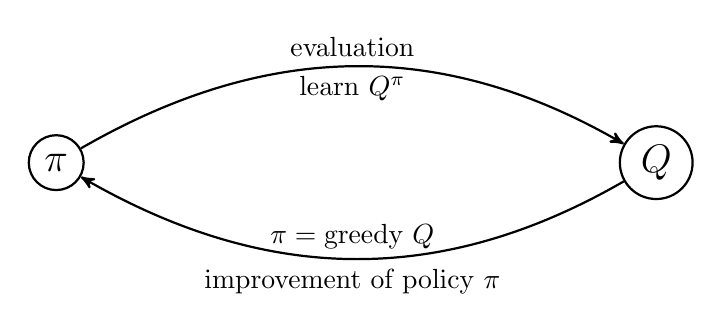
\begin{tikzpicture}[->,>=stealth',auto,node distance=3in,
        thick,main node/.style={circle,draw,font=\sffamily\Large\bfseries}]
    
        \node[main node] (pi) {$\pi$};
        \node[main node] (Q) [right of=pi] {$Q$};
        
        \draw [->] (pi) to [out=30,in=150] node [above]{evaluation} node [below]{learn $Q^\pi$} (Q);
        \draw [->] (Q) to [out=210,in=330] node [above]{$\pi = \text{greedy }Q$} node [below]{improvement of policy $\pi$} (pi);
    \end{tikzpicture}
    \caption{The relationship between the policy $\pi$ and the $Q$-function in generalized policy iteration.}
    \label{fig:gpi}
\end{figure}

\subsection{SARSA}

We next discuss SARSA (state-action-reward-next state-next action). The algorithm is as follows:

\begin{algorithm}
    \caption*{\textsc{SARSA}}
	\begin{algorithmic}[1]
    	\STATE \textbf{Initialize} $\hat{Q}^{\pi_0}$
    	\STATE \textbf{Generate} $S_0$
    	\STATE \textbf{Generate} $A_0$ using $\epsilon$-greedy policy: 
    	    $$\pi_0(a|s) = \prob{A_0=a|S_0=s} = 
    	    \begin{cases}
            \text{uniform action selection} & \text{with probability } \epsilon \\ 
            \argmax_{a'} \hat{Q}^{\pi_0} & \text{with probability } 1 - \epsilon \\ 
            \end{cases}$$
    	\FOR{$j \geq 1$}
    	    \STATE \textbf{Take action} $A_{j-1}=a$ and observe $S_j=s'$
    	    \STATE \textbf{Select action} $a'$ from the $\epsilon$-greedy $\hat{Q}^{\pi_{j - 1}}$ 
    	    \STATE \textbf{Update} $\hat{Q}$: $$\hat{Q}^{\pi_{j}} = \hat{Q}^{\pi_{j - 1}} + \alpha_j\left[\underbrace{R + \gamma \hat{Q}^{\pi_{j - 1}}(s', a')}_{\text{target}} - \hat{Q}^{\pi_{j - 1}}(s, a)\right]\mathbbm{1}_{S_{j-1}=s, A_{j-1}=a}$$
    	    \STATE \textbf{Set} $s \leftarrow s'$, $a \leftarrow a'$ 
    	\ENDFOR
    \end{algorithmic}
\end{algorithm}

At each iteration through the \textit{for} loop, SARSA makes one step toward learning the state-action value function that was just used to select the action, updating only a single state-action pair $s, a$. This is evident from the indicator at line 7. An interesting characteristic of this algorithm is the fact that we select a new action $a'$ at line 6 without learning anything, which is quite odd, since not performing updates before selecting the next action seems counterintuitive. This action $a'$ is chosen from $\pi_j$, the epsilon-greedy policy of $\hat{Q}^{\pi_{j-1}}$.

This is called \textit{``on-policy'' temporal difference control}. It's not quite on-policy, but our $\pi_{j-1}$ should be close to $\pi_j$. We are essentially tracking the current policy.

\subsection{Expected SARSA}

As stated in the SARSA algorithm, $R + \gamma \hat{Q}^{\pi_{j-1}}(s', a')$ is the target in our incremental update. However, as before, the target isn't perfect -- our selection of $a'$ adds noise to the target. We can reduce the variance of the target by using \textit{expected SARSA}, a slight modification of SARSA.

In expected SARSA, the update in line 7 of the original SARSA algorithm is slightly altered. The update becomes $$\hat{Q}^{\pi_{j}} = \hat{Q}^{\pi_{j - 1}} + \alpha_j\left[\underbrace{R + \gamma \sum_{b \in \mathcal{A}}\pi_j(b|s')\hat{Q}^{\pi_{j - 1}}(s', b)}_\text{new target} - \hat{Q}^{\pi_{j - 1}}(s, a)\right]\mathbbm{1}_{S_{j-1}=s, A_{j-1}=a},$$ where $\mathcal{A}$ is the space of actions. 

Since expected SARSA uses an expected $Q$-function over the action space rather than $Q(s',a')$, the new target (denoted above) is clearly lower variance. But the variance comparison if we take the max over $b$ (below) is uncertain. However, we do know that this slight alteration results in the $Q$-learning update!
$$\hat{Q}_j^{\pi^\star} = \hat{Q}_{j - 1}^{\pi^\star} + \alpha_j\left[\underbrace{R + \gamma \max_{b} \hat{Q}_{j - 1}^{\pi^\star}(s', b)}_\text{new target} - \hat{Q}^{\pi^\star}(s, a)\right]\mathbbm{1}_{S_{j-1}=s, A_{j-1}=a}$$

% if $\epsilon$ doesn't go to 0, then both $Q$ and $\pi$ may not converge?

% consider a gridworld where there's a giant chasm and a bridge. In an $\epsilon$-greedy algorithm, you'll sometimes walk off the bridge, even if you know it's bad, so the fact that you'll die will make you want to walk around the chasm

% discussion on regret of expected SARSA and Q-learning

\bibentry{suttonbarto, littman}

\bibliography{stat234}
\end{document}
